\makeatletter
\def\input@path{{../styles/}{../../styles/}{../../../styles/}{../}{../../}{../../../}}
\makeatother


\documentclass{ee122_pset}

% Assignment info
\author{\rule{3cm}{0.4pt}} % Name placeholder
\submitdate{\rule{3cm}{0.4pt}} % Submission date placeholder
\problemset{Problem Set \#11: Loop shaping-based controller design}
\renewcommand{\duedate}{April 23, 2026}
\shorttitle{Problem Set \#11}

\begin{document}
\problem{1} 
Consider the second-order plant
\[
G(s)=\frac{1}{s^2 + 6s + 5}.
\]

In Figure~\ref{fig:desiredloop}, you are given the desired loop gain magnitude plot for
\[
L(s)=C(s)G(s).
\]
Your goal is to design a compensator using loop-shaping ideas so that the loop transfer function approximately matches the desired magnitude plot.

\begin{figure}[h!]
    \centering
    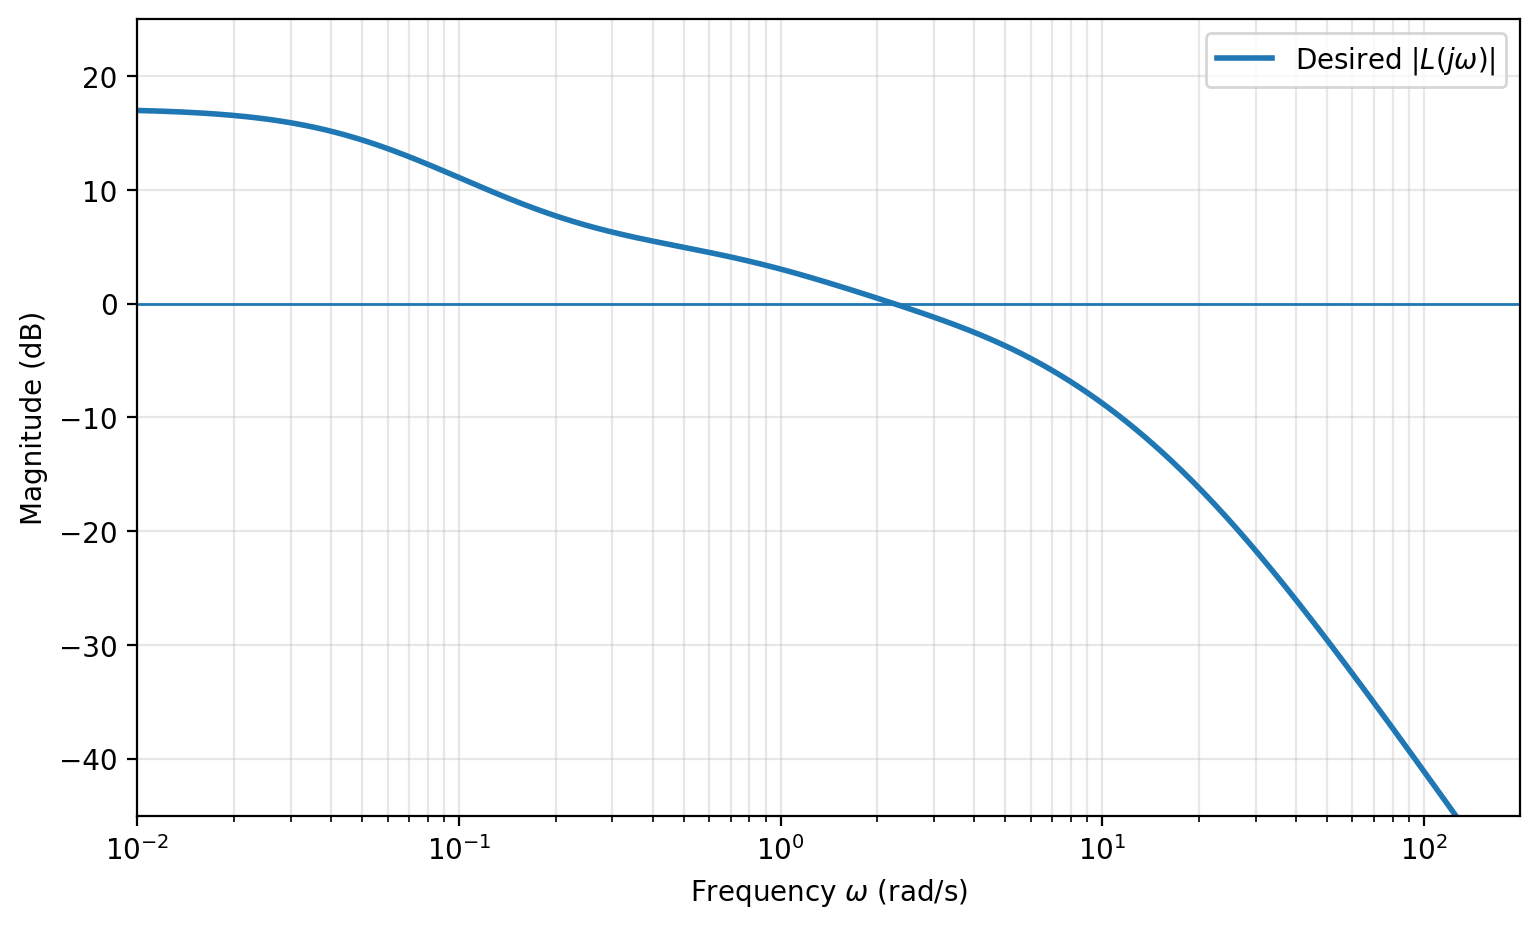
\includegraphics[width=0.82\textwidth]{desired_loop_gain.png}
    \caption{Desired loop-gain magnitude plot.}
    \label{fig:desiredloop}
\end{figure}

\problempart \textbf{[10 points]} Start from the plant \(G(s)\) and sketch its asymptotic Bode magnitude plot.
    
\problempart \textbf{[30 points]} From the desired loop-gain plot, determine how many additional poles and zeros must be contributed by the compensator. Write down the structure of the lead-lag compensator \(C(s)\) that you will use for this design.
    
\problempart \textbf{[10 points]} Estimate the break frequencies of the compensator by comparing the slope changes in the desired plot against the known break frequencies of the plant.
    
\problempart \textbf{[10 points]} Identify which part of your compensator acts as the \emph{lag} portion and which part acts as the \emph{lead} portion.
    
\problempart \textbf{[10 points]} Estimate the gain \(K\) needed so that the compensated loop transfer function
    \[
    L(s)=C(s)G(s)
    \]
    matches the desired magnitude plot.
    
\problempart \textbf{[10 points]} Write your final compensator \(C(s)\) explicitly.
    
\problempart \textbf{[20 points]} Plot the Bode magnitude of your designed loop transfer function and compare it against the desired plot.
    
\end{document}